%
% This is a borrowed LaTeX template file for lecture notes for CS267,
% Applications of Parallel Computing, UCBerkeley EECS Department.
% Now being used for CMU's 10725 Fall 2012 Optimization course
% taught by Geoff Gordon and Ryan Tibshirani.  When preparing 
% LaTeX notes for this class, please use this template.
%
% To familiarize yourself with this template, the body contains
% some examples of its use.  Look them over.  Then you can
% run LaTeX on this file.  After you have LaTeXed this file then
% you can look over the result either by printing it out with
% dvips or using xdvi. "pdflatex template.tex" should also work.
%

\documentclass[twoside]{article}
\setlength{\oddsidemargin}{0.25 in}
\setlength{\evensidemargin}{-0.25 in}
\setlength{\topmargin}{-0.6 in}
\setlength{\textwidth}{6.5 in}
\setlength{\textheight}{8.5 in}
\setlength{\headsep}{0.75 in}
\setlength{\parindent}{0 in}
\setlength{\parskip}{0.1 in}

%
% ADD PACKAGES here:
%

\usepackage{amsmath,amsfonts,graphicx}

%
% The following commands set up the lecnum (lecture number)
% counter and make various numbering schemes work relative
% to the lecture number.
%
\newcounter{lecnum}
\renewcommand{\thepage}{\thelecnum-\arabic{page}}
\renewcommand{\thesection}{\thelecnum.\arabic{section}}
\renewcommand{\theequation}{\thelecnum.\arabic{equation}}
\renewcommand{\thefigure}{\thelecnum.\arabic{figure}}
\renewcommand{\thetable}{\thelecnum.\arabic{table}}

%
% The following macro is used to generate the header.
%
\newcommand{\lecture}[4]{
   \pagestyle{myheadings}
   \thispagestyle{plain}
   \newpage
   \setcounter{lecnum}{#1}
   \setcounter{page}{1}
   \noindent
   \begin{center}
   \framebox{
      \vbox{\vspace{2mm}
    \hbox to 6.28in { {\bf EE402 - Discrete Time Systems
	\hfill Spring 2018} }
       \vspace{4mm}
       \hbox to 6.28in { {\Large \hfill Lecture #1 \hfill} }
       \vspace{2mm}
       \hbox to 6.28in { {\it Lecturer: #2 \hfill } }
      \vspace{2mm}}
   }
   \end{center}
   \markboth{Lecture #1}{Lecture #1}

   \vspace*{4mm}
}
%
% Convention for citations is authors' initials followed by the year.
% For example, to cite a paper by Leighton and Maggs you would type
% \cite{LM89}, and to cite a paper by Strassen you would type \cite{S69}.
% (To avoid bibliography problems, for now we redefine the \cite command.)
% Also commands that create a suitable format for the reference list.
\renewcommand{\cite}[1]{[#1]}
\def\beginrefs{\begin{list}%
        {[\arabic{equation}]}{\usecounter{equation}
         \setlength{\leftmargin}{2.0truecm}\setlength{\labelsep}{0.4truecm}%
         \setlength{\labelwidth}{1.6truecm}}}
\def\endrefs{\end{list}}
\def\bibentry#1{\item[\hbox{[#1]}]}

%Use this command for a figure; it puts a figure in wherever you want it.
%usage: \fig{NUMBER}{SPACE-IN-INCHES}{CAPTION}
\newcommand{\fig}[3]{
			\vspace{#2}
			\begin{center}
			Figure \thelecnum.#1:~#3
			\end{center}
	}
% Use these for theorems, lemmas, proofs, etc.
\newtheorem{theorem}{Theorem}[lecnum]
\newtheorem{lemma}[theorem]{Lemma}
\newtheorem{proposition}[theorem]{Proposition}
\newtheorem{claim}[theorem]{Claim}
\newtheorem{corollary}[theorem]{Corollary}
\newtheorem{definition}[theorem]{Definition}
\newenvironment{proof}{{\bf Proof:}}{\hfill\rule{2mm}{2mm}}

% **** IF YOU WANT TO DEFINE ADDITIONAL MACROS FOR YOURSELF, PUT THEM HERE:

\begin{document}

% Lecture Details
\lecture{2}{Asst. Prof. M. Mert Ankarali}

\par

\section*{Big Picture of EE402}

In this course, the main focus will be on continuous-time systems that
are controlled (sampled and actuated) by a digital computer
interface. Such a discrete-time control system consists of four major
parts as illustrated in Fig.~\ref{fig:introblock},
 
\begin{enumerate}
  \item \textit{The plant} is a continuous-time dynamical system 
  \item Analog-to-Digital Converter (ADC)
  \item Controller ($\mu P$), a microprocessor/microcontroller
    with a ``real-time'' OS 
 \item Digital-to-Analog Converter (DAC) 
\end{enumerate}

\begin{figure}[h]
    \centering
      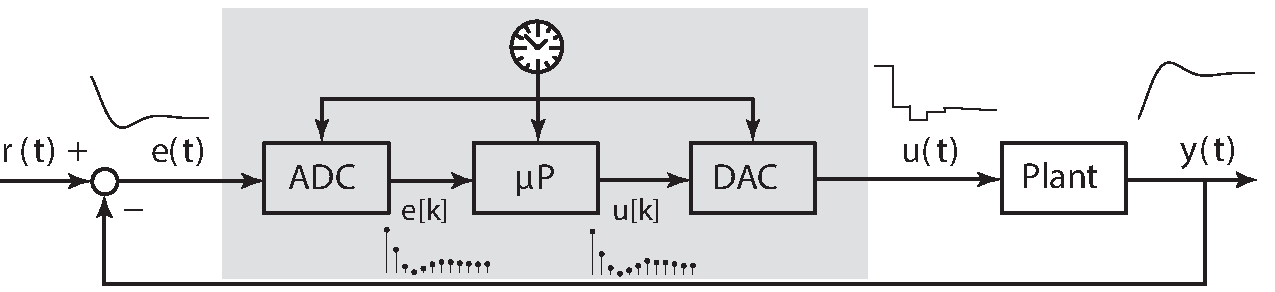
\includegraphics[width=0.99\textwidth]{introblock}
    \caption{Block diagram of a digital control system}
    \label{fig:introblock}
\end{figure}

Most of the time, the plant is modeled as a ``smooth'' continuous dynamical
system. In this course, we will focus on LTI systems. Rhus, we will assume
that (unless otherwise is given), the plant is a continuous LTI
plant model with a transfer function of $G_c(s)$ for which both the
input and output are continuous time signals. 

The ``digital'' blocks inside the closed-loop block diagram structure are 
ADC, the Controller, and DAC. It is generally assumed (design
requirement) that all blocks shares a common ``hard real time'' clock.

A general ADC is a device that converts an analog signal to a digital
signal. In this course, we will model the ADC block as an \textit{ideal sampler}
for which the input is a continious-time signal, $e(t)$, and the output 
is a discrete-time signal, $e[k]$, where the relation between the
continuous- and discrete-time signals are given as
%
\begin{align*}
  e(kT) = e[k] , \ k \in \mathbb{Z}^+, 
\end{align*}
%
where constant $T$ is the \textit{sampling time}. 

The microcontroller/microprocessor processes some set of digital input signals
to produce some set of digital output signals. The outputs are defined
at only some specified instances defined by the real-time clock. In this
course, we will model the $\mu P$ block as an ideal discrete-time LTI
system for which both the input and output are discrete-time
signals, with a transfer function of $G_c(z)$.

The DAC is a device that converts a digital signal to an analog
signal. In this course we assume that it is an ideal \textit{Hold}
element for which the input signal is a discrete-time signal, where as
output is a continuous-time signal. The most commonly used
\textit{Hold} system is ZOH (Zero-Order-Hold) which is a mapping 
defined by the following relation
%
\begin{align*}
  u(t) = u[k] , \ \mathrm{for} t \in [kT , (k+1)T )
\end{align*}
%
Higher-order holds available but seldom used.

The idealized and simplified block-diagram structure is given in Fig.

\begin{figure}[h]
    \centering
      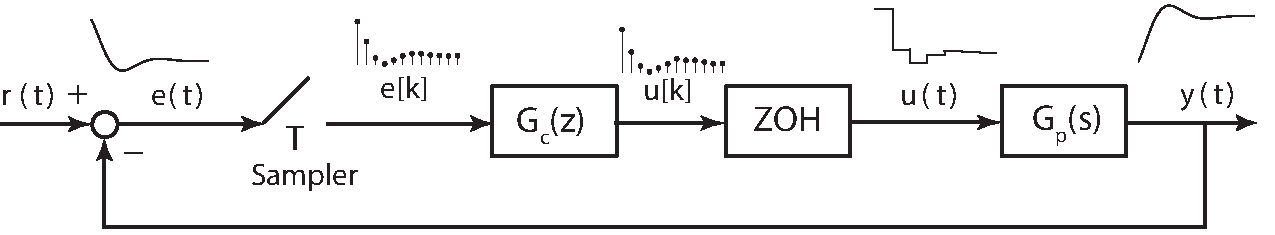
\includegraphics[width=0.99\textwidth]{idealblock}
    \caption{Block diagram of an LTI discrete-time control system}
    \label{fig:introblock}
\end{figure}

\textbf{Major challenge:} Loop contains both continuous-time and discrete-time parts.

\section*{Sampling}

\begin{figure}[h]
    \centering
      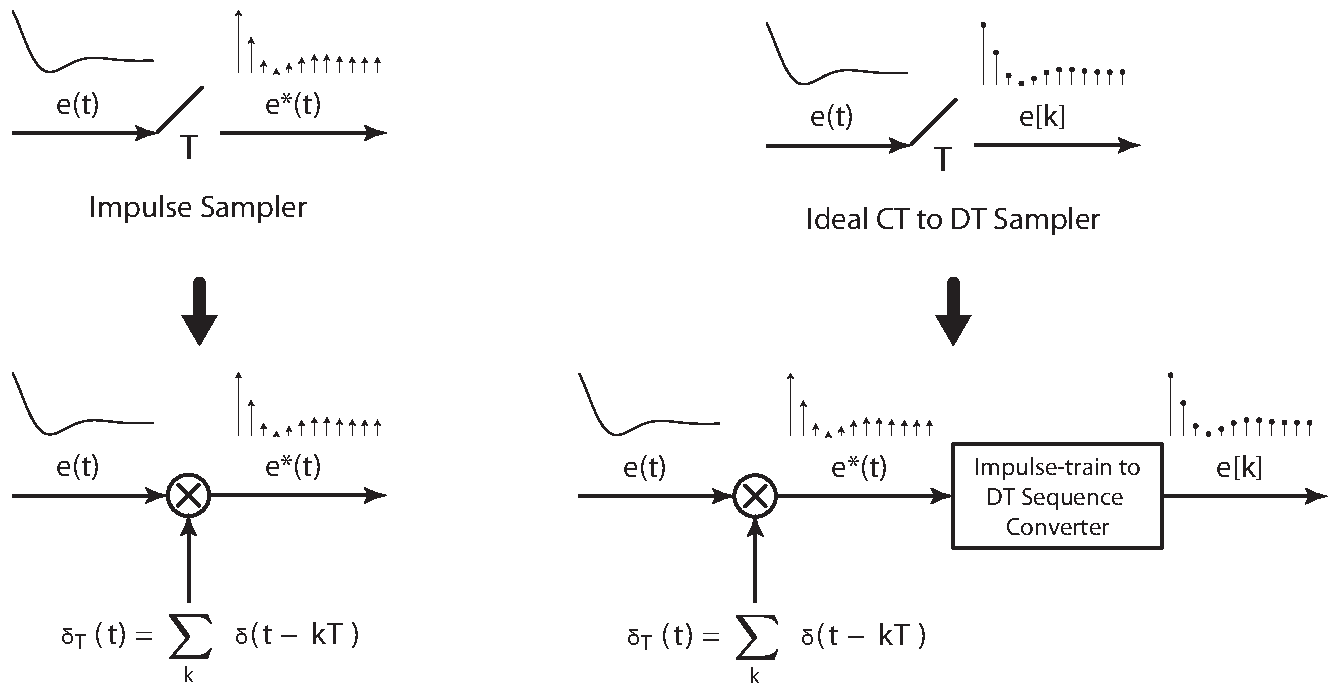
\includegraphics[width=0.99\textwidth]{sampling}
    \caption{Two different ideal samplers}
    \label{fig:sampling}
\end{figure}

Fig.~\ref{fig:sampling} illustrates two different ideal sampler (both
of them will be covered in this course. Firs column is an
\textit{impulse sampler} for which the output is a continuous signal
but it is composed of trains of impulses (impulse train). Second one
is an ideal complete CT-to-DT sampler which convertes the impulse train
into DT sequence.

The output of the impulse sampler, $x*(t)$, can be represented with
the following infinte summations
%
\begin{align*}
  x^*(t) &= \sum\limits_{k=0}^{\infty} x(kT) \delta(t - kT) =
          \sum\limits_{k=0}^{\infty} x[k] \delta(t - kT) 
\\ \mathrm{or}& \\
  x^*(t) &= x(0) \delta(t) + x(T) \delta(t - T) + \cdots +
 x(k T) \delta(t - kT) + \cdots \\
&= x[0] \delta(t) + x[1] \delta(t - T) + \cdots +
 x[k] \delta(t - kT) + \cdots 
\end{align*}
 %
Now let's consider the Laplace transform of $x^*(t)$
%
\begin{align*}
  X^*(s) &= \mathcal{L} \lbrace x^*(t) \rbrace = \mathcal{L}
  \left\lbrace \sum\limits_{k=0}^{\infty} x(kT) \delta(t - kT)
  \right\rbrace
= \sum\limits_{k=0}^{\infty} x(kT) \mathcal{L}
  \left\lbrace \delta(t - kT)
  \right\rbrace 
\\
  &= \sum\limits_{k=0}^{\infty} x(kT) 
  \int\limits_{t=0}^{\infty} \delta(t - kT) e^{-s t} dt
    = \sum\limits_{k=0}^{\infty} x(kT) e^{-s kT}
 = \sum\limits_{k=0}^{\infty} x[k] e^{-s kT}
\end{align*}
%
Now let's define a map in complex domain
such that 
%
\begin{align*}
z = e^{Ts} \ \mathrm{or} \ s = \frac{1}{T} \ln z
\end{align*}
%
Then we have
%
\begin{align*}
  X^*(s)|_{s = (1/T) ln z} = \sum\limits_{k=0}^{\infty} x[k] z^{-k} 
\end{align*}
%
where 
%
\begin{align*}
  X(z) = \mathcal{Z} \lbrace x[k] \rbrace = \sum\limits_{k=0}^{\infty} x[k] z^{-k} 
\end{align*}

\section*{Z-transform}
%
Z-transform of a (causal) discrete time signal $x[k]$ is given by 
%
\begin{align*}
  X(z) = \mathcal{Z} \lbrace x[k] \rbrace = \sum\limits_{k=0}^{\infty} x[k] z^{-k} 
\end{align*}
%
If $x[k]$ is a sampled signal from a continuous time signal $x(t)$
with a sampling time of $T$, we (abuse of notation) also use the
following notation
%
\begin{align*}
  X(z) = \mathcal{Z} \lbrace x(kT) \rbrace = \mathcal{Z} \lbrace x^*(t) \rbrace 
\end{align*}
% 
\subsection*{Z-transforms of elementary functions}

We assume that all signals are causal thus $t \in \mathbb{R}^+$
and $k \in \mathbb{Z}^+$

Unit-step function $x(t) = 1$ and thus $x(kT) = x[k] = 1$, the
Z-transform is given by
%
\begin{align*}
 X(z) = \sum\limits_{k=0}^{\infty} z^{-k} = \frac{1}{1 - z^{-1}} =
  \frac{z}{z - 1}
\end{align*}
%
Unit-ramp function $x(t) = t$ and thus $x(kT) = x[k] = kT$, the
Z-transform is given by
%
\begin{align*}
 X(z) &= \sum\limits_{k=0}^{\infty} kT z^{-k} = T (z^{-1} + 2 z^{-2}  +
  3 z^{-3}  + \cdots) 
= T z (z^{-2} + 2 z^{-3}  +
  3 z^{-4}  + \cdots) \\ &= T z \frac{d}{dz} \left( 
 \int (z^{-2} + 2 z^{-3}  + 3 z^{-4}  + \cdots) dz \right)
= T z \frac{d}{dz} \left( 
  -(z^{-1} + z^{-2}  + z^{-3}  + \cdots) \right)
\\
&= T z \frac{d}{dz} \left(  \frac{-1}{z-1} \right)  = \frac{T
  z}{(z-1)^2} =
\frac{T z^{-1}}{(1 - z^{-1})^2} 
\end{align*}
%
Exponential sequence $x[k] = a^k$
%
\begin{align*}
 X(z) = \sum\limits_{k=0}^{\infty} a^k z^{-k} =
  \sum\limits_{k=0}^{\infty} \left( \frac{z}{a} \right)^{-k} = 
\frac{1}{1 - a z^{-1}} = \frac{z}{z - a}
\end{align*}
%
Exponential function $x(t) = e^{b t}$ and thus $x(k T) = x(k) = e^{b T
  k}$
%
\begin{align*}
 X(z) = \sum\limits_{k=0}^{\infty} e^{b T k} z^{-k} = \sum\limits_{k=0}^{\infty} (e^{b T})^k z^{-k}
= \frac{1}{1 - e^{b T} z^{-1}} = \frac{z}{z - e^{b T}}
\end{align*}
%
Cosine function $x(t) = \cos (\omega t)$, and thus $x(k T) = x(k) =
\cos (\omega T k)$
%
\begin{align*}
\cos (\omega T k) &= \frac{1}{2} \left( e^{j \omega T k} + e^{-j \omega T k} \right)
 X(z) = \frac{1}{2} \left( \frac{z}{z - e^{j \omega T}} +  \frac{z}{z
  - e^{-j \omega T}} \right) = 
\frac{1}{2} \frac{z(z - e^{-j \omega T}) + z(z - e^{j \omega T})}{(z
  - e^{-j \omega T}) (z - e^{j \omega T})}
\\
&= \frac{1}{2} \frac{2 z^2 - z(e^{-j \omega T} + e^{j \omega T})}{z^2
  -z (e^{-j \omega T} + e^{j \omega T}) + 1}
= \frac{z^2 - z \cos(\omega T)}{z^2 - z 2 \cos (\omega T)+ 1}
\\ &= \frac{1 - z^{-1} \cos(\omega T)}{1 - z^{- 1} 2 \cos (\omega T) + z^{-2}}
\end{align*}
%

\subsection*{Properties and Theorems of the Z-transform}

\textbf{Linearity}
%
\begin{align*}
  x(k) = \alpha f(k) + \beta g(k) \ \rightarrow X(z) = \alpha F(z) +
  \beta G(z) \ , \forall \ \alpha, \ \beta, \ f(k), \ \& \ g(k)
\end{align*}

\textbf{Multiplication by $a^k$}
%
\begin{align*}
\mathcal{Z} \lbrace a^k x[k] \rbrace &= \sum\limits_{k=0}^{\infty} 
  a^k x[k] z^{-k} = \sum\limits_{k=0}^{\infty}  x[k] (z/a)^{-k} 
\\
\mathcal{Z} \lbrace a^k x[k] \rbrace &= X(z/a)
\end{align*}

\textbf{Complex translation theorem}
%
Let $y(t) = e^{-a t} x(t)$ and $X(z) = \mathcal{z} \lbrace x(k T)
\rbrace$, then
%
\begin{align*}
\mathcal{Z} \lbrace y(k T) \rbrace = \mathcal{Z} \lbrace e^{-a T k}
  x(k T) \rbrace = X(e^{a T} z)
\end{align*}

\textbf{Shifting theorem}
%
Let $x(t)$ be a causal CT signal, thus we have $x(t) = 0$ for 
$t < 0$. Similarly sampled DT signal has the property $x[nk] = 0$ for $k <
0$. For the sake of simplicity lets work on the sampled (i.e. DT)
signal. Let
%
\begin{align*}
\mathcal{Z} \lbrace x^*(t) \rbrace = \mathcal{Z} \lbrace x[k] \rbrace = X(z)
\end{align*}

\textit{Shifting right by N (Causal shifting):} Let $y[k] = x[k - N]$,
then
\begin{align*}
\mathcal{Z} \lbrace y[k]\rbrace = \sum\limits_{k=0}^{\infty} y[k] z^{-k}
= \sum\limits_{k=0}^{\infty} x[k - N] z^{-k} = \sum\limits_{k=N}^{\infty} x[k - N] z^{-k}
\end{align*}
%
Let $k = m + N$ then 
%
\begin{align*}
\mathcal{Z} \lbrace y[k]\rbrace &= \sum\limits_{m=0}^{\infty} x[m]
  z^{-(m+N)} = z^{-N} \sum\limits_{m=0}^{\infty} x[m]
  z^{-m}  
\\
\mathcal{Z} \lbrace x[k-N]\rbrace &= z^{-N} X(z)
\end{align*}

\textit{Shifting left by N (Non-causal shifting) \& Bilateral Z
  transform:}  Let $y[k] = x[k + N]$,
%
\begin{align*}
\mathcal{Z} \lbrace x[k+N]\rbrace &= \sum\limits_{k=-\infty}^{\infty}
  x[k +N] z^{-k} = \sum\limits_{m=-\infty}^{\infty} x[m] z^{-(m-N)} 
= z^N \sum\limits_{m=-\infty}^{\infty} x[m] z^{-m} 
\\
\mathcal{Z} \lbrace x[k+N]\rbrace &= z^N X(z)
\end{align*}

\textit{Shifting left by N (Non-causal shifting) \& Unilateral Z
  transform:}  Let $y[k] = x[k + N]$,
%
\begin{align*}
\mathcal{Z} \lbrace x[k+N]\rbrace &= \sum\limits_{k=0}^{\infty}
  x[k + N] z^{-k} 
\end{align*}
%
Let $k = m - N$ then 
%
\begin{align*}
\mathcal{Z} \lbrace x[k+N]\rbrace &= \sum\limits_{m=N}^{\infty}
  x[m] z^{-(m-N)} = z^N \sum\limits_{m=N}^{\infty}
  x[m] z^{-m} = z^N \left( \sum\limits_{k=0}^{\infty}
  x[k] z^{-k} - \sum\limits_{k=0}^{N-1} x[k] z^{-k} \right)
\\ 
\mathcal{Z} \lbrace x[k+N]\rbrace &= z^N \left( X(z) -
                                    \sum\limits_{k=0}^{N-1} x[k]
                                    z^{-k} \right)
\end{align*}
%
From this equation we can obtain
\begin{align*}
\mathcal{Z} \lbrace x[k+1]\rbrace &= z X(z) - z x[0]
\\
\mathcal{Z} \lbrace x[k+2]\rbrace &= z^2 X(z) - z^2 x[0] - z x[1]
\\
\vdots &
\end{align*}

\textbf{Example 1.} Let $u[k]$ be the unit-step function. Compute
$\mathcal{Z} \lbrace u[k-1] \rbrace$ both directly and using the shifting property.
%
\begin{align*}
  \mathcal{Z} \lbrace u[k-1] \rbrace = \frac{z^{-1}}{1 - z^{-1}}
\end{align*}
%


\textbf{Example 2.} Let $y[k] = \sum\limits_{n=0}^{k} x[k]$ where $k
\in \mathbb{Z}^+$. Compute $Y(z)$ in terms of $X(z)$ using the
shifting theorem.
%
\begin{align*}
 Y(z) = \frac{1}{1 - z^{-1}} X(z)
\end{align*}
%

\textbf{Initial Value Theorem}
%
Let $X(z) = \mathcal{Z} \lbrace x[n] \rbrace$ and if the following limit exists, 
then the initial value of $x[0]$ or $x(0)$ is given by
%
\begin{align*}
x[0] = \lim_{z \to \infty} X(z)
\end{align*}
%
Indeed the proof is very easy
%
\begin{align*}
\lim_{z \to \infty} X(z) = \lim_{z \to \infty} \left[
  \sum\limits_{k=0}^{\infty} x(k) z^{-k} \right] = \lim_{z \to \infty} \left[ x(0) + x(1) z^{-1} +
  x(2) z^{-2} + \cdots \right]
 = x(0)
\end{align*}
%

\textbf{Final Value Theorem}

Let's assume that $x(kT)$ or $x[k]$ is a convergent sequence (DT
signal). Then the final value theorem states that 
%
\begin{align*}
\lim_{k \to \infty} x[k] = \lim_{z \to 1} (1 - z^{-1}) X(z)
\end{align*}
%

\textbf{Proof:} Let's take the Z transform of $x[k] - x[k-1]$
%
\begin{align*}
  \mathcal{Z} \lbrace x[k] - x[k-1] \rbrace &=
  \sum\limits_{k=0}^{\infty} \left( x[k] - x[k-1] \right) z^{-k}
\\
 X(z) - X(z) z^{-1} &= \left( x[0] \left( 1 - z^{-1} \right) + x[1]
                      \left( z^{-1} - z^{-2} \right) + x[2] \left(
                      z^{-2} - z^{-3} \right) + x[3] \left(
                      z^{-3} - z^{-4} \right) + \cdots \right)  +
                      \lim_{k \to \infty} x[k] z^{-k}
\\
\lim_{z \to 1} X(z) \left( 1 - z^{-1} \right) &= \left( 0 + 0 + \cdots
                                                \right) + \lim_{z \to
                                                1} \lim_{k \to \infty}
                                                x[k] z^{-k}
\\
\lim_{z \to 1} X(z) \left( 1 - z^{-1} \right) &= \lim_{k \to \infty} x[k] 
\end{align*}

\textbf{Complex Differentiation Theorem}

Consider
%
\begin{align*}
\frac{d}{dz} X(z) &= \frac{d}{dz} \left[ \sum\limits_{k=0}^{\infty}
  x[k] z^{-k} \right] = \sum\limits_{k=0}^{\infty}
  x[k] \frac{d}{dz} z^{-k} = \sum\limits_{k=0}^{\infty}
  (-k) x[k] z^{-k-1} 
\\
- z \frac{d}{dz} X(z) &= \sum\limits_{k=0}^{\infty}
  k x[k] z^{-k} 
\\
- z \frac{d}{dz} X(z) &= \mathcal{Z} \lbrace k x[k] \rbrace
\end{align*}
%
In general 
%
\begin{align*}
(- z)^m \frac{d}{dz^m} X(z) &= \mathcal{Z} \lbrace k^m x[k] \rbrace
\end{align*}

\textbf{Example 3.} Find the Z-transform of the unit ramp function,
$r[k] = k \ , k \in \mathbb{Z}^+$ by applying the Complex Differentiation Theorem to the
Z-transform of the unit step function. 


\textbf{Real Convolution Theorem}
%
Let $f[k]$ and $g[k]$ are causal signals and associated Z transforms
are $F(z)$ and $G(z)$ respectively.
%
The DT convolution operator is defined as
%
\begin{align*}
 f[n] \ast g[n] = \sum\limits_{k=0}^{n} f[n-k] g[k]
\end{align*}
%
Real Convolution Theorem states that
%
\begin{align*}
 \mathcal{Z} \lbrace f[n] \ast g[n] \rbrace = F(z) G(z)
\end{align*}
%
\textbf{Proof}

\begin{align*}
 \mathcal{Z} \lbrace f[n] \ast g[n] \rbrace =
  \sum\limits_{n=0}^{\infty} \left [ \sum\limits_{k=0}^{n} f[n-k] g[k]
  \right] z^{-n}
\end{align*}
%
Since we know that $f[m] = 0$ for $m<0$, we can stretch the upper
limit of the sum as
%
\begin{align*}
 \mathcal{Z} \lbrace f[n] \ast g[n] \rbrace =
  \sum\limits_{n=0}^{\infty} \left [ \sum\limits_{k=0}^{\infty} f[n-k] g[k]
  \right] z^{-n}
 = \sum\limits_{k=0}^{\infty} \sum\limits_{n=0}^{\infty}  f[n-k] g[k] z^{-n}
\end{align*}
%
Let $n = m + k$ then 
%
\begin{align*}
 \mathcal{Z} \lbrace f[n] \ast g[n] \rbrace &=
  \sum\limits_{k=0}^{\infty}  \sum\limits_{m=-k}^{\infty} f[m] g[k]
  z^{-m} z^{-k}
  = \sum\limits_{k=0}^{\infty} g[k] z^{-k} \sum\limits_{m=0}^{\infty}
  f[m] z^{-m} 
\\
 \mathcal{Z} \lbrace f[n] \ast g[n] \rbrace &= F(z) G(z) 
\end{align*}
%

\section*{The Inverse Z-transform}

\begin{enumerate}
 \item Direct division method
 \item Z-tranform tables \& partial-fraction expansion 
 \item ``Simulation'' method
 \item Inversion integral method
\end{enumerate}

\subsection*{Direct division}

Direct division (or long division) method uses the fact that $X(z)$
can be expressed as
%
\begin{align*}
  X(z) = \sum\limits_{k=0}^{\infty} x[k] z^{-k} = x(0) + x(1) z^{-1} +
  x(2) z^{-2} + x(3) z^{-3} + \cdots
\end{align*}
%
The goal is finding the power series expansion of $X(z)$ using the
long division approach. Here we assume that $X(z)$ cane be represnted
as a ratio of two polynomials in $z$ (or $z^{-1}$) 

\begin{align*}
  X(z) = \frac{b_0 z^m + b_1 z^{m-1} + \cdots + b_m}{z^n + a_1
  z^{n-1} + \cdots + a_n} = 
\frac{b_0 z^{-n+m} + b_1 z^{-n+m-1} + \cdots + b_m z^{-n}}{1 + a_1
  z^{-1} + \cdots + a_n z^{-n}} 
\end{align*}

For the direct division method it is easer to work when the
polynomials are written interms of powers of $z^{-1}$.

\textbf{Example 4.} Find the inverse Z-transform of $X(z) =
\frac{z^{-1}}{1 - 2 z^{-1} + z^{-2}}$.  

\begin{center}
  \begin{minipage}[h]{0.9\linewidth}
    \begin{center}
      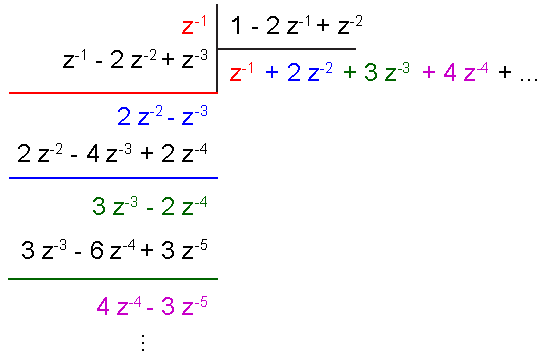
\includegraphics[width=0.7\textwidth]{directdivision}
    \end{center}
  \end{minipage}
\end{center}
%
Thus, 
%
\begin{align*} 
  X(z) &= 0 + 1 z^{-1} + 2 z^{-2} + 3 z^{-3} + 4 z^{-4} + ...  \\
 \downarrow
\\
  x[k] &= 0 \delta[k] + 1 \delta[k-1] + 2 \delta[k-2] + 3 \delta[k-3] + 4
  \delta[k-4] + ...  = k
\end{align*}
%
\subsection*{Partial Fraction Expansion}
%
In most applications $X(z)$ can be re-written in terms of
poles and zeros as
%
\begin{align*}
    X(z) &= b_0 \frac{(z- z_1) \cdots (z- z_m)}{(z- p_1) \cdots (z-p_n)} \ \ (m \leq n)
\end{align*}
%
Specific (but extremely common) case 
%
\begin{align*}
    \frac{X(z)}{z} &= \sum\limits_{i=1}^n \frac{a_i}{(z- p_i)} 
\end{align*}
%
where all poles are distinct and simple order. We can compute 
each $a_i$ using
%
\begin{align*}
    a_i &= \lim_{z \to p_i} \left[ (z- p_i) \frac{X(z)}{z}  \right]
\end{align*}
%
\textbf{Example 5.} Find the  inverse Z-transform of $X(z) =
\frac{(1-b)z}{(z-1) (z-b)}$. Solution:
%
\begin{align*}
    \frac{X(z)}{z} &= \frac{(1-b)}{(z-1) (z-b)} = \frac{a_1}{z-1} + 
                     \frac{a_2}{z-b} \\
    a_1 &= \lim_{z \to 1} \left[ (z -1) \frac{X(z)}{z} \right] = 1 \\
    a_2 &= \lim_{z \to b} \left[ (z -b) \frac{X(z)}{z} \right] = -1 \\
   X(z) &= \frac{z}{z-1} - \frac{z}{z-b} \\
   x[k] &= 1 - b^k
\end{align*}
%
Now let's assume that $\frac{X(z)}{z}$ has double pole at $p_1$ and
all other poles are distinct 
%
\begin{align*}
    \frac{X(z)}{z} &= \frac{c_1}{z- p_1}  + \frac{c_2}{(z- p_1)^2} + \cdots
\end{align*}
%
It is easy to show that
%
\begin{align*}
    c_2 &= \lim_{z \to p_1} \left[ (z- p_1)^2 \frac{X(z)}{z}  \right]
\end{align*}
%
It is also possible to show that
%
\begin{align*}
    c_1 &= \lim_{z \to p_1} \left\lbrace \frac{d}{dz}\left[ (z- p_1)^2
          \frac{X(z)}{z}  \right] \right \rbrace
\end{align*}
%
\textbf{Example 6.} Find the  inverse Z-transform $X(z) =
\frac{2 z^2 - 3 z}{(z-1)^2}$. Solution:
%
\begin{align*}
    \frac{X(z)}{z} &=  \frac{c_1}{z- 1}  + \frac{c_2}{(z-1)^2} \\
    c_1 &= \lim_{z \to 1} \frac{d}{z} \left[ (z -1)^2 \frac{X(z)}{z} \right] = 2 \\
    c_2 &= \lim_{z \to 1} \left[ (z -1)^2 \frac{X(z)}{z} \right] = -1 \\
   x[k] &= 2 - k
\end{align*}
%
\textbf{Example 7.} Find the  inverse Z-transform $X(z) =
\frac{(1-b)}{(z-1) (z-b)}$. Solution:
%
\begin{align*}
    X(z) &= \frac{(1-b)}{(z-1) (z-b)} = \frac{a_1}{z-1} + 
                     \frac{a_2}{z-b} \\
    a_1 &= \lim_{z \to 1} \left[ (z - 1) X(z) \right] = 1 \\
    a_2 &= \lim_{z \to b} \left[ (z - b) X(z) \right] = -1 \\
   X(z) &= z^{-1} \left( \frac{z}{z-1} - \frac{z}{z-b} \right) \\
   x[k] &= [ 1 - b^{k-1} ] u[k-1]
\end{align*}
%
\textbf{Example 8.} Find the  inverse Z-transform $X(z) =
\frac{z^2 - 2}{(z-1) (z-2)}$. Solution:
%
\begin{align*}
X(z) &= \frac{z^2 - 2}{z^2 - 3 z + 2} = 1 + \frac{3z - 4}{z^2 - 3 z + 2}
\\
    X(z) &= 1 + \frac{a_1}{z-1} + \frac{a_2}{z-2} \\
    a_1 &= \lim_{z \to 1} \left[ (z -1) X(z) \right] = 1 \\
    a_2 &= \lim_{z \to 2} \left[ (z -2) X(z) \right] = 2 \\
   X(z) &= 1 +\frac{1}{z-1} + \frac{2}{z-2} = \frac{1}{z-1} +
          \frac{z}{z-2} \\
   x[k] &= 1 + 2^k - \delta[k] 
\end{align*}
%

% **** This ENDS THE EXAMPLES. DON'T DELETE THE FOLLOWING LINE:
\end{document}